\section{Datenanalyse}
\subsection{Detektor Bilder}
\begin{frame}
	\frametitle{Elektronen Events}
	\begin{columns}[T] % align columns
		\begin{column}{.54\textwidth}
			\begin{figure}
				\centering
				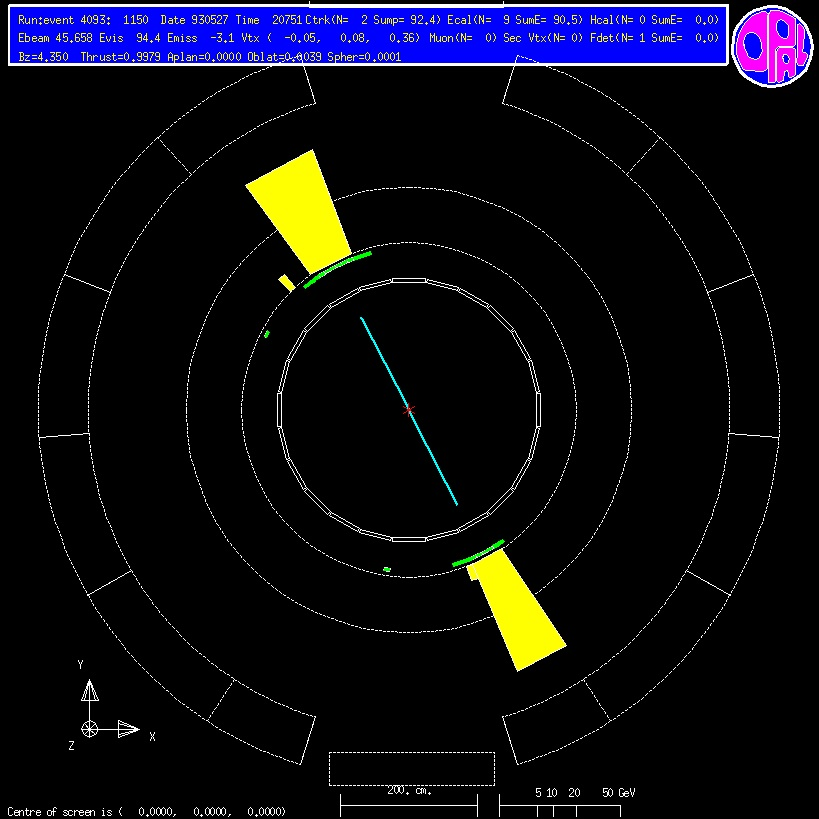
\includegraphics[width=1.0\linewidth]{graphics/electronopal}
			\end{figure}
		\end{column}%
		\hfill%
		\begin{column}{.42\textwidth}
			\begin{center}
				\begin{itemize}
					\item Meistens 2 geladene Spuren
					\item Energiedeposition im EM-Kalorimeter
				\end{itemize}
			\end{center}
		\end{column}%
	\end{columns}
\end{frame}

\begin{frame}
	\frametitle{Myonen Events}
	\begin{columns}[T] % align columns
		\begin{column}{.54\textwidth}
			\begin{figure}
				\centering
				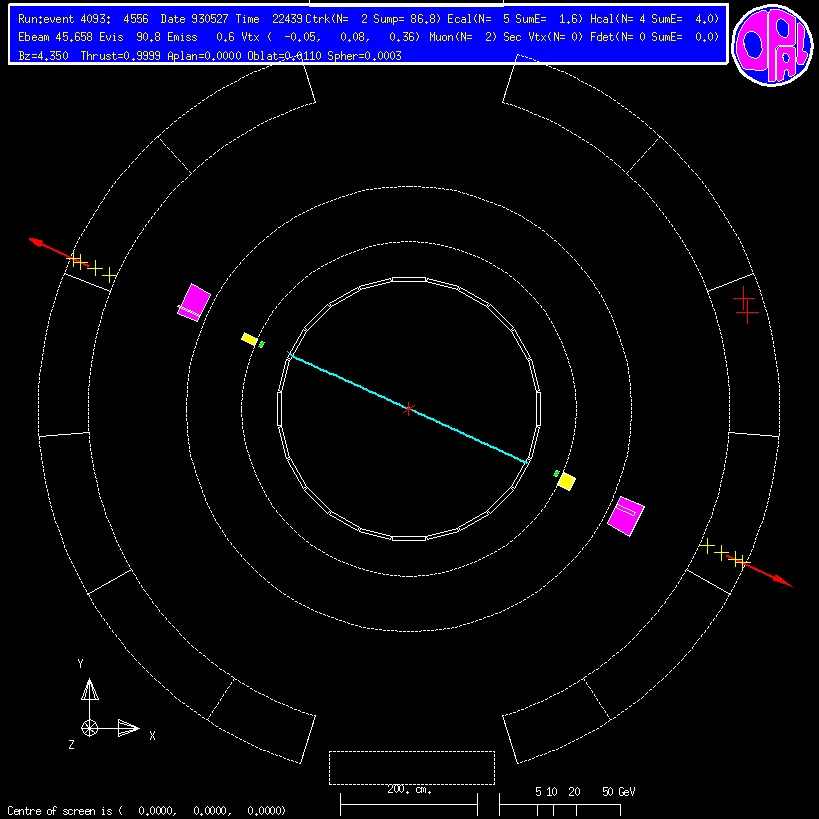
\includegraphics[width=1.0\linewidth]{graphics/muonopal}
			\end{figure}
		\end{column}%
		\hfill%
		\begin{column}{.42\textwidth}
			\begin{center}
				\begin{itemize}
					\item 2 geladene Spuren
					\item Wenig Deposition in EM- und Hadronenkalorimeter
					\item Vektorspuren in Muonenkammer
				\end{itemize}
			\end{center}
		\end{column}%
	\end{columns}
	
\end{frame}
\begin{frame}
	\frametitle{Tauonen Events}
	\begin{columns}[T] % align columns
		\begin{column}{.54\textwidth}
			\begin{figure}
				\centering
				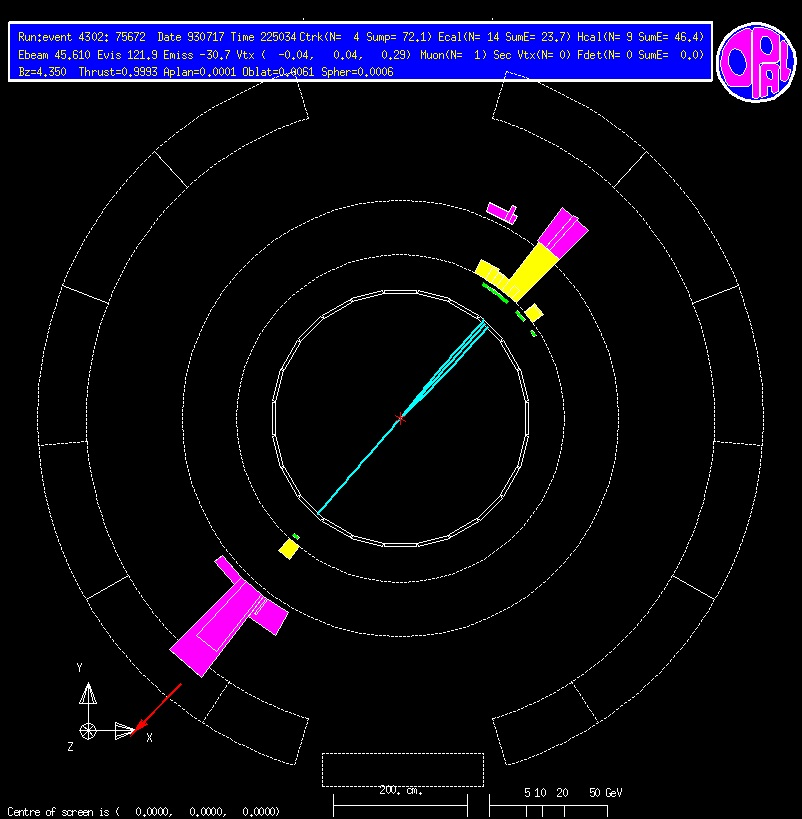
\includegraphics[width=1.0\linewidth]{graphics/tauonopal}
			\end{figure}
		\end{column}%
		\hfill%
		\begin{column}{.42\textwidth}
			\begin{center}
				\begin{itemize}
					\item Tauonen sehr kurzlebig \\$\Rightarrow$ Zerfallsprodukte
					\item $64.79\%$ Zerfall in 2-4 $\pi^{0,\pm}$ und $\nu_\tau$
					\item Sonst $e^{\pm}$/$\mu^{\pm}$ und $\nu_\tau$
					\item Hier: 3 bzw. 1 geladenes Pion
					\item Einzelnes Myon aus Hadronenkalorimeter
				\end{itemize}
			\end{center}
		\end{column}%
	\end{columns}
	
\end{frame}
\begin{frame}
	\frametitle{Quark Events}
	\begin{columns}[T] % align columns
		\begin{column}{.54\textwidth}
			\begin{figure}
				\centering
				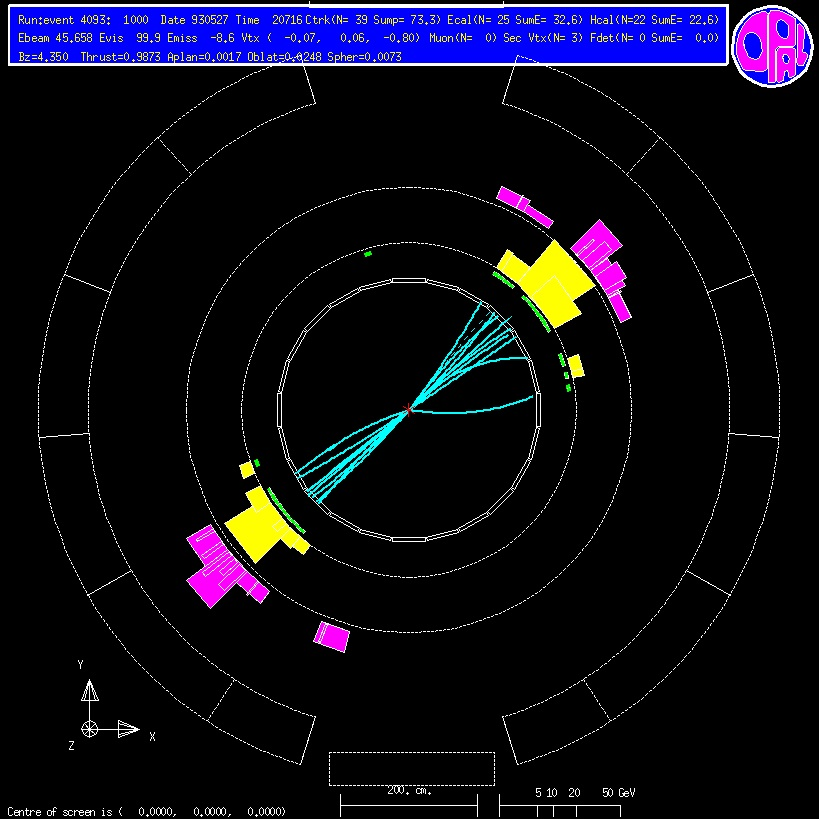
\includegraphics[width=1.0\linewidth]{graphics/quarkopal}
			\end{figure}
		\end{column}%
		\hfill%
		\begin{column}{.42\textwidth}
			\begin{center}
				\begin{itemize}
					\item Hadronen Jets
					\item bis zu 35 Spuren
					\item Energie in EM- und Hadronenkalorimeter
				\end{itemize}
			\end{center}
		\end{column}%
	\end{columns}
	
\end{frame}
\subsection{Daten der Monte-Carlo Simulation}
\begin{frame}
	\frametitle{Monte-Carlo und Detektorsimulationen}
	\begin{center}
		\begin{itemize}
			\item Benötigt um Events zu klassifizieren
			\item 
		\end{itemize}
	\end{center}
\end{frame}
\subsection{Cuts und Aufbereitung der Daten}
\begin{frame}
	\frametitle{E\_Ecal Histogramm}
	
\end{frame}

\begin{frame}
	\frametitle{Zwei Photon Untergrund}
	
\end{frame}

\begin{frame}
	\frametitle{Reinheit der Cuts}
	
\end{frame}
\begin{frame}
	\frametitle{Die Effizienzmatrix}
	
\end{frame}
\begin{frame}
	\frametitle{Die Inverse Effizienzmatrix}
	
\end{frame}

\subsection{Auswertung der aufgearbeiteten Daten}
\begin{frame}
	\frametitle{Wirkungsquerschnitte}

\end{frame}
\begin{frame}
	\frametitle{Masse des $Z^0$ Bosons}
	
\end{frame}
\begin{frame}
	\frametitle{Zerfallsbreiten}
	
\end{frame}
\begin{frame}
	\frametitle{Leptonenuniversalität}
	
\end{frame}
\begin{frame}
	\frametitle{Neutrinogenerationen}
	
\end{frame}
\begin{frame}
	\frametitle{Vorwärts-Rückwärts Asymmetrie}
	
\end{frame}
\begin{frame}
	\frametitle{Berechnung des Weinberg Winkels}
	
\end{frame}





